\documentclass[1p]{elsarticle_modified}
%\bibliographystyle{elsarticle-num}

%\usepackage[colorlinks]{hyperref}
%\usepackage{abbrmath_seonhwa} %\Abb, \Ascr, \Acal ,\Abf, \Afrak
\usepackage{amsfonts}
\usepackage{amssymb}
\usepackage{amsmath}
\usepackage{amsthm}
\usepackage{scalefnt}
\usepackage{amsbsy}
\usepackage{kotex}
\usepackage{caption}
\usepackage{subfig}
\usepackage{color}
\usepackage{graphicx}
\usepackage{xcolor} %% white, black, red, green, blue, cyan, magenta, yellow
\usepackage{float}
\usepackage{setspace}
\usepackage{hyperref}

\usepackage{tikz}
\usetikzlibrary{arrows}

\usepackage{multirow}
\usepackage{array} % fixed length table
\usepackage{hhline}

%%%%%%%%%%%%%%%%%%%%%
\makeatletter
\renewcommand*\env@matrix[1][\arraystretch]{%
	\edef\arraystretch{#1}%
	\hskip -\arraycolsep
	\let\@ifnextchar\new@ifnextchar
	\array{*\c@MaxMatrixCols c}}
\makeatother %https://tex.stackexchange.com/questions/14071/how-can-i-increase-the-line-spacing-in-a-matrix
%%%%%%%%%%%%%%%

\usepackage[normalem]{ulem}

\newcommand{\msout}[1]{\ifmmode\text{\sout{\ensuremath{#1}}}\else\sout{#1}\fi}
%SOURCE: \msout is \stkout macro in https://tex.stackexchange.com/questions/20609/strikeout-in-math-mode

\newcommand{\cancel}[1]{
	\ifmmode
	{\color{red}\msout{#1}}
	\else
	{\color{red}\sout{#1}}
	\fi
}

\newcommand{\add}[1]{
	{\color{blue}\uwave{#1}}
}

\newcommand{\replace}[2]{
	\ifmmode
	{\color{red}\msout{#1}}{\color{blue}\uwave{#2}}
	\else
	{\color{red}\sout{#1}}{\color{blue}\uwave{#2}}
	\fi
}

\newcommand{\Sol}{\mathcal{S}} %segment
\newcommand{\D}{D} %diagram
\newcommand{\A}{\mathcal{A}} %arc


%%%%%%%%%%%%%%%%%%%%%%%%%%%%%5 test

\def\sl{\operatorname{\textup{SL}}(2,\Cbb)}
\def\psl{\operatorname{\textup{PSL}}(2,\Cbb)}
\def\quan{\mkern 1mu \triangleright \mkern 1mu}

\theoremstyle{definition}
\newtheorem{thm}{Theorem}[section]
\newtheorem{prop}[thm]{Proposition}
\newtheorem{lem}[thm]{Lemma}
\newtheorem{ques}[thm]{Question}
\newtheorem{cor}[thm]{Corollary}
\newtheorem{defn}[thm]{Definition}
\newtheorem{exam}[thm]{Example}
\newtheorem{rmk}[thm]{Remark}
\newtheorem{alg}[thm]{Algorithm}

\newcommand{\I}{\sqrt{-1}}
\begin{document}

%\begin{frontmatter}
%
%\title{Boundary parabolic representations of knots up to 8 crossings}
%
%%% Group authors per affiliation:
%\author{Yunhi Cho} 
%\address{Department of Mathematics, University of Seoul, Seoul, Korea}
%\ead{yhcho@uos.ac.kr}
%
%
%\author{Seonhwa Kim} %\fnref{s_kim}}
%\address{Center for Geometry and Physics, Institute for Basic Science, Pohang, 37673, Korea}
%\ead{ryeona17@ibs.re.kr}
%
%\author{Hyuk Kim}
%\address{Department of Mathematical Sciences, Seoul National University, Seoul 08826, Korea}
%\ead{hyukkim@snu.ac.kr}
%
%\author{Seokbeom Yoon}
%\address{Department of Mathematical Sciences, Seoul National University, Seoul, 08826,  Korea}
%\ead{sbyoon15@snu.ac.kr}
%
%\begin{abstract}
%We find all boundary parabolic representation of knots up to 8 crossings.
%
%\end{abstract}
%\begin{keyword}
%    \MSC[2010] 57M25 
%\end{keyword}
%
%\end{frontmatter}

%\linenumbers
%\tableofcontents
%
\newcommand\colored[1]{\textcolor{white}{\rule[-0.35ex]{0.8em}{1.4ex}}\kern-0.8em\color{red} #1}%
%\newcommand\colored[1]{\textcolor{white}{ #1}\kern-2.17ex	\textcolor{white}{ #1}\kern-1.81ex	\textcolor{white}{ #1}\kern-2.15ex\color{red}#1	}

{\Large $\underline{10_{116}~(K10a_{120})}$}

\setlength{\tabcolsep}{10pt}
\renewcommand{\arraystretch}{1.6}
\vspace{1cm}\begin{tabular}{m{100pt}>{\centering\arraybackslash}m{274pt}}
\multirow{5}{120pt}{
	\centering
	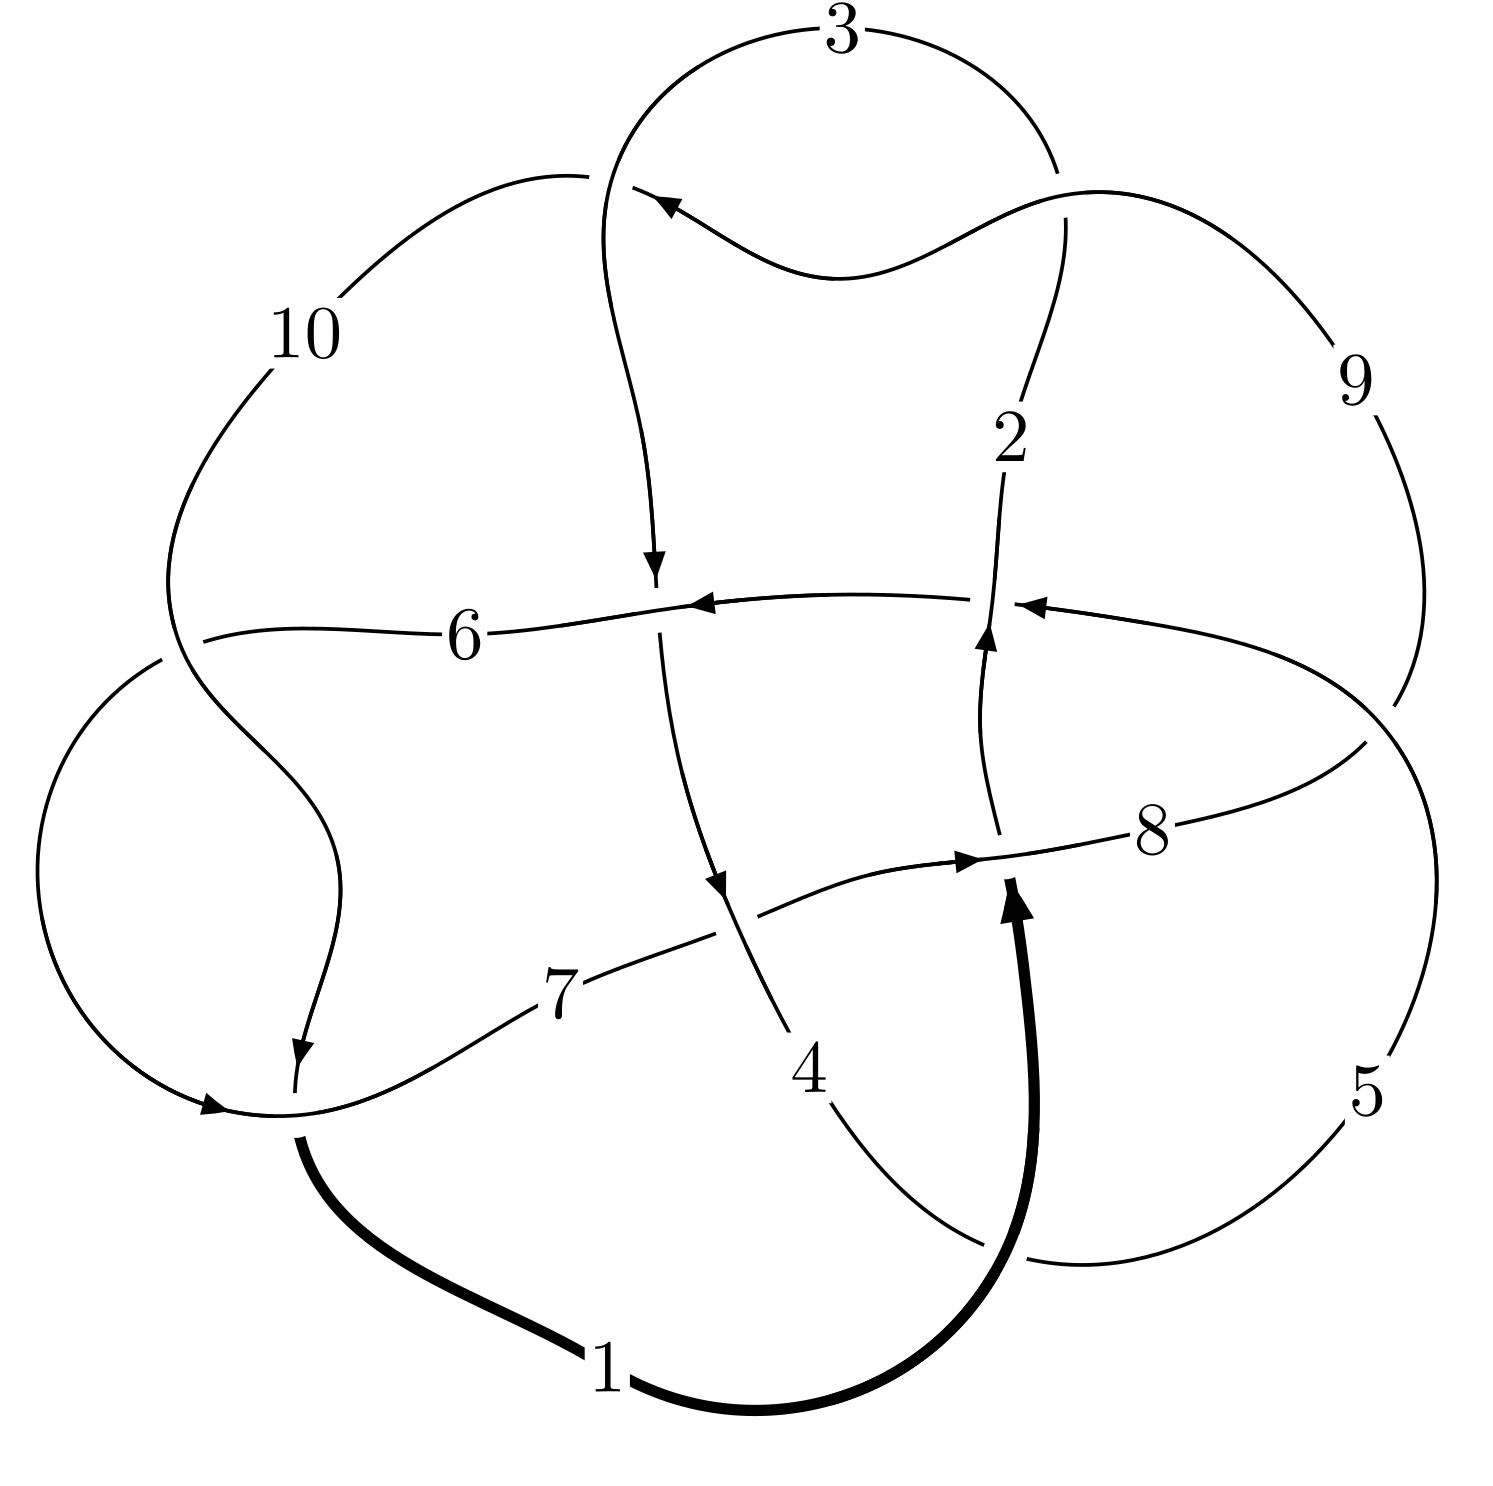
\includegraphics[width=112pt]{../../../GIT/diagram.site/Diagrams/png/200_10_116.png}\\
\ \ \ A knot diagram\footnotemark}&
\allowdisplaybreaks
\textbf{Linearized knot diagam} \\
\cline{2-2}
 &
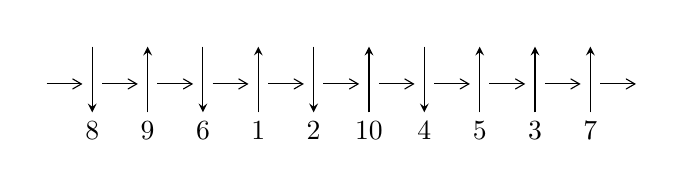
\begin{tikzpicture}[x=20pt, y=17pt]
	% nodes
	\node (C0) at (0, 0) {};
	\node (C1) at (1, 0) {};
	\node (C1U) at (1, +1) {};
	\node (C1D) at (1, -1) {8};

	\node (C2) at (2, 0) {};
	\node (C2U) at (2, +1) {};
	\node (C2D) at (2, -1) {9};

	\node (C3) at (3, 0) {};
	\node (C3U) at (3, +1) {};
	\node (C3D) at (3, -1) {6};

	\node (C4) at (4, 0) {};
	\node (C4U) at (4, +1) {};
	\node (C4D) at (4, -1) {1};

	\node (C5) at (5, 0) {};
	\node (C5U) at (5, +1) {};
	\node (C5D) at (5, -1) {2};

	\node (C6) at (6, 0) {};
	\node (C6U) at (6, +1) {};
	\node (C6D) at (6, -1) {10};

	\node (C7) at (7, 0) {};
	\node (C7U) at (7, +1) {};
	\node (C7D) at (7, -1) {4};

	\node (C8) at (8, 0) {};
	\node (C8U) at (8, +1) {};
	\node (C8D) at (8, -1) {5};

	\node (C9) at (9, 0) {};
	\node (C9U) at (9, +1) {};
	\node (C9D) at (9, -1) {3};

	\node (C10) at (10, 0) {};
	\node (C10U) at (10, +1) {};
	\node (C10D) at (10, -1) {7};
	\node (C11) at (11, 0) {};

	% arrows
	\draw[->,>={angle 60}]
	(C0) edge (C1) (C1) edge (C2) (C2) edge (C3) (C3) edge (C4) (C4) edge (C5) (C5) edge (C6) (C6) edge (C7) (C7) edge (C8) (C8) edge (C9) (C9) edge (C10) (C10) edge (C11) ;	\draw[->,>=stealth]
	(C1U) edge (C1D) (C2D) edge (C2U) (C3U) edge (C3D) (C4D) edge (C4U) (C5U) edge (C5D) (C6D) edge (C6U) (C7U) edge (C7D) (C8D) edge (C8U) (C9D) edge (C9U) (C10D) edge (C10U) ;
	\end{tikzpicture} \\
\hhline{~~} \\& 
\textbf{Solving Sequence} \\ \cline{2-2} 
 &
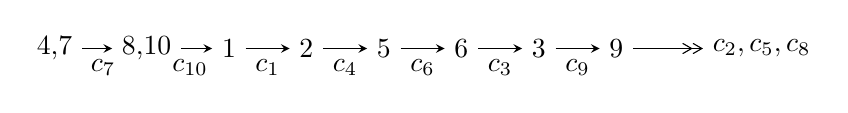
\begin{tikzpicture}[x=28pt, y=7pt]
	% node
	\node (A0) at (-1/8, 0) {4,7};
	\node (A1) at (17/16, 0) {8,10};
	\node (A2) at (17/8, 0) {1};
	\node (A3) at (25/8, 0) {2};
	\node (A4) at (33/8, 0) {5};
	\node (A5) at (41/8, 0) {6};
	\node (A6) at (49/8, 0) {3};
	\node (A7) at (57/8, 0) {9};
	\node (C1) at (1/2, -1) {$c_{7}$};
	\node (C2) at (13/8, -1) {$c_{10}$};
	\node (C3) at (21/8, -1) {$c_{1}$};
	\node (C4) at (29/8, -1) {$c_{4}$};
	\node (C5) at (37/8, -1) {$c_{6}$};
	\node (C6) at (45/8, -1) {$c_{3}$};
	\node (C7) at (53/8, -1) {$c_{9}$};
	\node (A8) at (9, 0) {$c_{2},c_{5},c_{8}$};

	% edge
	\draw[->,>=stealth]	
	(A0) edge (A1) (A1) edge (A2) (A2) edge (A3) (A3) edge (A4) (A4) edge (A5) (A5) edge (A6) (A6) edge (A7) ;
	\draw[->>,>={angle 60}]	
	(A7) edge (A8);
\end{tikzpicture} \\ 

\end{tabular} \\

\footnotetext{
The image of knot diagram is generated by the software ``\textbf{Draw programme}" developed by Andrew Bartholomew(\url{http://www.layer8.co.uk/maths/draw/index.htm\#Running-draw}), where we modified some parts for our purpose(\url{https://github.com/CATsTAILs/LinksPainter}).
}\phantom \\ \newline 
\centering \textbf{Ideals for irreducible components\footnotemark of $X_{\text{par}}$} 
 
\begin{align*}
I^u_{1}&=\langle 
-3043 u^{15}+828 u^{14}+\cdots+761 b-4040,\;1027 u^{15}-1203 u^{14}+\cdots+761 a+653,\\
\phantom{I^u_{1}}&\phantom{= \langle  }u^{16}- u^{15}+u^{14}-2 u^{13}+7 u^{12}-8 u^{11}+7 u^{10}-6 u^9+6 u^8+7 u^7-24 u^6+32 u^5-27 u^4+20 u^3-12 u^2+5 u-1\rangle \\
I^u_{2}&=\langle 
6.18811\times10^{62} u^{35}-2.36237\times10^{62} u^{34}+\cdots+2.97721\times10^{61} b+3.69879\times10^{62},\\
\phantom{I^u_{2}}&\phantom{= \langle  }-3.31586\times10^{63} u^{35}+1.45172\times10^{63} u^{34}+\cdots+2.97721\times10^{61} a-1.62016\times10^{63},\;u^{36}- u^{35}+\cdots+10 u-1\rangle \\
I^u_{3}&=\langle 
u^3+u^2+b+1,\;- u^4-2 u^3- u^2+a- u-1,\;u^5+u^4+u^3+2 u^2+u+1\rangle \\
\\
\end{align*}
\raggedright * 3 irreducible components of $\dim_{\mathbb{C}}=0$, with total 57 representations.\\
\footnotetext{All coefficients of polynomials are rational numbers. But the coefficients are sometimes approximated in decimal forms when there is not enough margin.}
\newpage
\renewcommand{\arraystretch}{1}
\centering \section*{I. $I^u_{1}= \langle -3043 u^{15}+828 u^{14}+\cdots+761 b-4040,\;1027 u^{15}-1203 u^{14}+\cdots+761 a+653,\;u^{16}- u^{15}+\cdots+5 u-1 \rangle$}
\flushleft \textbf{(i) Arc colorings}\\
\begin{tabular}{m{7pt} m{180pt} m{7pt} m{180pt} }
\flushright $a_{4}=$&$\begin{pmatrix}0\\u\end{pmatrix}$ \\
\flushright $a_{7}=$&$\begin{pmatrix}1\\0\end{pmatrix}$ \\
\flushright $a_{8}=$&$\begin{pmatrix}1\\u^2\end{pmatrix}$ \\
\flushright $a_{10}=$&$\begin{pmatrix}-1.34954 u^{15}+1.58081 u^{14}+\cdots+8.93955 u-0.858081\\3.99869 u^{15}-1.08804 u^{14}+\cdots-20.1130 u+5.30880\end{pmatrix}$ \\
\flushright $a_{1}=$&$\begin{pmatrix}2.64915 u^{15}+0.492773 u^{14}+\cdots-11.1735 u+4.45072\\3.99869 u^{15}-1.08804 u^{14}+\cdots-20.1130 u+5.30880\end{pmatrix}$ \\
\flushright $a_{2}=$&$\begin{pmatrix}2.30092 u^{15}+1.16163 u^{14}+\cdots-4.12089 u+2.28384\\3.80158 u^{15}-2.29435 u^{14}+\cdots-22.0644 u+5.62943\end{pmatrix}$ \\
\flushright $a_{5}=$&$\begin{pmatrix}6.61367 u^{15}-1.88436 u^{14}+\cdots-31.2247 u+9.78844\\5.73456 u^{15}-1.78449 u^{14}+\cdots-25.8279 u+7.37845\end{pmatrix}$ \\
\flushright $a_{6}=$&$\begin{pmatrix}3.15112 u^{15}-1.87516 u^{14}+\cdots-22.0039 u+7.48752\\4.22733 u^{15}+0.231275 u^{14}+\cdots-12.4494 u+3.57687\end{pmatrix}$ \\
\flushright $a_{3}=$&$\begin{pmatrix}4.03022 u^{15}-1.97503 u^{14}+\cdots-25.4008 u+8.89750\\5.50329 u^{15}-0.279895 u^{14}+\cdots-20.7175 u+6.72799\end{pmatrix}$ \\
\flushright $a_{9}=$&$\begin{pmatrix}-5.53482 u^{15}+2.16689 u^{14}+\cdots+32.0053 u-10.3167\\-7.74901 u^{15}+1.81603 u^{14}+\cdots+34.5848 u-9.98160\end{pmatrix}$\\&\end{tabular}
\flushleft \textbf{(ii) Obstruction class $= -1$}\\~\\
\flushleft \textbf{(iii) Cusp Shapes $= \frac{13489}{761} u^{15}+\frac{456}{761} u^{14}+\cdots-\frac{54502}{761} u+\frac{17914}{761}$}\\~\\
\newpage\renewcommand{\arraystretch}{1}
\flushleft \textbf{(iv) u-Polynomials at the component}\newline \\
\begin{tabular}{m{50pt}|m{274pt}}
Crossings & \hspace{64pt}u-Polynomials at each crossing \\
\hline $$\begin{aligned}c_{1}\end{aligned}$$&$\begin{aligned}
&u^{16}+8 u^{15}+\cdots-22 u-4
\end{aligned}$\\
\hline $$\begin{aligned}c_{2},c_{6},c_{9}\\c_{10}\end{aligned}$$&$\begin{aligned}
&u^{16}-8 u^{14}+\cdots+4 u+1
\end{aligned}$\\
\hline $$\begin{aligned}c_{3}\end{aligned}$$&$\begin{aligned}
&u^{16}-12 u^{15}+\cdots+112 u-16
\end{aligned}$\\
\hline $$\begin{aligned}c_{4},c_{8}\end{aligned}$$&$\begin{aligned}
&u^{16}- u^{15}+\cdots+5 u-1
\end{aligned}$\\
\hline $$\begin{aligned}c_{5},c_{7}\end{aligned}$$&$\begin{aligned}
&u^{16}- u^{15}+\cdots+5 u-1
\end{aligned}$\\
\hline
\end{tabular}\\~\\
\newpage\renewcommand{\arraystretch}{1}
\flushleft \textbf{(v) Riley Polynomials at the component}\newline \\
\begin{tabular}{m{50pt}|m{274pt}}
Crossings & \hspace{64pt}Riley Polynomials at each crossing \\
\hline $$\begin{aligned}c_{1}\end{aligned}$$&$\begin{aligned}
&y^{16}-2 y^{15}+\cdots-44 y+16
\end{aligned}$\\
\hline $$\begin{aligned}c_{2},c_{6},c_{9}\\c_{10}\end{aligned}$$&$\begin{aligned}
&y^{16}-16 y^{15}+\cdots-18 y+1
\end{aligned}$\\
\hline $$\begin{aligned}c_{3}\end{aligned}$$&$\begin{aligned}
&y^{16}+46 y^{14}+\cdots+1632 y+256
\end{aligned}$\\
\hline $$\begin{aligned}c_{4},c_{8}\end{aligned}$$&$\begin{aligned}
&y^{16}-11 y^{15}+\cdots-17 y+1
\end{aligned}$\\
\hline $$\begin{aligned}c_{5},c_{7}\end{aligned}$$&$\begin{aligned}
&y^{16}+y^{15}+\cdots- y+1
\end{aligned}$\\
\hline
\end{tabular}\\~\\
\newpage\flushleft \textbf{(vi) Complex Volumes and Cusp Shapes}
$$\begin{array}{c|c|c}  
\text{Solutions to }I^u_{1}& \I (\text{vol} + \sqrt{-1}CS) & \text{Cusp shape}\\
 \hline 
\begin{aligned}
u &= \phantom{-}0.848485 + 0.598766 I \\
a &= -0.483988 - 0.792063 I \\
b &= \phantom{-}1.362100 + 0.075359 I\end{aligned}
 & \phantom{-}7.97491 + 0.20600 I & \phantom{-}9.94793 + 0.07278 I \\ \hline\begin{aligned}
u &= \phantom{-}0.848485 - 0.598766 I \\
a &= -0.483988 + 0.792063 I \\
b &= \phantom{-}1.362100 - 0.075359 I\end{aligned}
 & \phantom{-}7.97491 - 0.20600 I & \phantom{-}9.94793 - 0.07278 I \\ \hline\begin{aligned}
u &= \phantom{-}0.846121 + 0.652012 I \\
a &= -0.284195 + 0.129063 I \\
b &= \phantom{-}0.014022 + 0.906951 I\end{aligned}
 & -2.23601 - 4.95570 I & -0.99614 + 6.15512 I \\ \hline\begin{aligned}
u &= \phantom{-}0.846121 - 0.652012 I \\
a &= -0.284195 - 0.129063 I \\
b &= \phantom{-}0.014022 - 0.906951 I\end{aligned}
 & -2.23601 + 4.95570 I & -0.99614 - 6.15512 I \\ \hline\begin{aligned}
u &= \phantom{-}0.664815 + 0.989330 I \\
a &= \phantom{-}1.38574 + 1.59724 I \\
b &= -1.227900 - 0.015479 I\end{aligned}
 & \phantom{-}6.88399 - 4.31481 I & \phantom{-}8.84422 + 5.32763 I \\ \hline\begin{aligned}
u &= \phantom{-}0.664815 - 0.989330 I \\
a &= \phantom{-}1.38574 - 1.59724 I \\
b &= -1.227900 + 0.015479 I\end{aligned}
 & \phantom{-}6.88399 + 4.31481 I & \phantom{-}8.84422 - 5.32763 I \\ \hline\begin{aligned}
u &= -1.20069\phantom{ +0.000000I} \\
a &= \phantom{-}0.395416\phantom{ +0.000000I} \\
b &= \phantom{-}0.206535\phantom{ +0.000000I}\end{aligned}
 & -2.54477\phantom{ +0.000000I} & -11.1320\phantom{ +0.000000I} \\ \hline\begin{aligned}
u &= -0.207234 + 0.684921 I \\
a &= \phantom{-}0.548174 - 0.525931 I \\
b &= \phantom{-}0.034860 - 0.480524 I\end{aligned}
 & \phantom{-}0.24918 + 1.55875 I & \phantom{-}1.96281 - 3.40867 I \\ \hline\begin{aligned}
u &= -0.207234 - 0.684921 I \\
a &= \phantom{-}0.548174 + 0.525931 I \\
b &= \phantom{-}0.034860 + 0.480524 I\end{aligned}
 & \phantom{-}0.24918 - 1.55875 I & \phantom{-}1.96281 + 3.40867 I \\ \hline\begin{aligned}
u &= -0.539685 + 1.175220 I \\
a &= -1.351880 + 0.225032 I \\
b &= \phantom{-}1.48126 + 0.46974 I\end{aligned}
 & \phantom{-}8.92084 + 7.21911 I & \phantom{-}9.60333 - 5.50334 I\\
 \hline 
 \end{array}$$\newpage$$\begin{array}{c|c|c}  
\text{Solutions to }I^u_{1}& \I (\text{vol} + \sqrt{-1}CS) & \text{Cusp shape}\\
 \hline 
\begin{aligned}
u &= -0.539685 - 1.175220 I \\
a &= -1.351880 - 0.225032 I \\
b &= \phantom{-}1.48126 - 0.46974 I\end{aligned}
 & \phantom{-}8.92084 - 7.21911 I & \phantom{-}9.60333 + 5.50334 I \\ \hline\begin{aligned}
u &= \phantom{-}0.435669 + 0.469034 I \\
a &= \phantom{-}1.43102 + 0.27627 I \\
b &= -0.975942 - 0.412090 I\end{aligned}
 & \phantom{-}1.82506 + 0.80819 I & \phantom{-}2.13059 - 1.11047 I \\ \hline\begin{aligned}
u &= \phantom{-}0.435669 - 0.469034 I \\
a &= \phantom{-}1.43102 - 0.27627 I \\
b &= -0.975942 + 0.412090 I\end{aligned}
 & \phantom{-}1.82506 - 0.80819 I & \phantom{-}2.13059 + 1.11047 I \\ \hline\begin{aligned}
u &= \phantom{-}0.491705\phantom{ +0.000000I} \\
a &= \phantom{-}1.58325\phantom{ +0.000000I} \\
b &= \phantom{-}1.37840\phantom{ +0.000000I}\end{aligned}
 & \phantom{-}7.98963\phantom{ +0.000000I} & \phantom{-}11.0630\phantom{ +0.000000I} \\ \hline\begin{aligned}
u &= -1.19368 + 1.15575 I \\
a &= \phantom{-}1.265790 - 0.496149 I \\
b &= -1.48086 - 0.47484 I\end{aligned}
 & \phantom{-}7.3807 + 15.4239 I & \phantom{-}6.04190 - 8.21765 I \\ \hline\begin{aligned}
u &= -1.19368 - 1.15575 I \\
a &= \phantom{-}1.265790 + 0.496149 I \\
b &= -1.48086 + 0.47484 I\end{aligned}
 & \phantom{-}7.3807 - 15.4239 I & \phantom{-}6.04190 + 8.21765 I\\
 \hline 
 \end{array}$$\newpage\newpage\renewcommand{\arraystretch}{1}
\centering \section*{II. $I^u_{2}= \langle 6.19\times10^{62} u^{35}-2.36\times10^{62} u^{34}+\cdots+2.98\times10^{61} b+3.70\times10^{62},\;-3.32\times10^{63} u^{35}+1.45\times10^{63} u^{34}+\cdots+2.98\times10^{61} a-1.62\times10^{63},\;u^{36}- u^{35}+\cdots+10 u-1 \rangle$}
\flushleft \textbf{(i) Arc colorings}\\
\begin{tabular}{m{7pt} m{180pt} m{7pt} m{180pt} }
\flushright $a_{4}=$&$\begin{pmatrix}0\\u\end{pmatrix}$ \\
\flushright $a_{7}=$&$\begin{pmatrix}1\\0\end{pmatrix}$ \\
\flushright $a_{8}=$&$\begin{pmatrix}1\\u^2\end{pmatrix}$ \\
\flushright $a_{10}=$&$\begin{pmatrix}111.375 u^{35}-48.7610 u^{34}+\cdots-994.024 u+54.4186\\-20.7849 u^{35}+7.93485 u^{34}+\cdots+169.058 u-12.4237\end{pmatrix}$ \\
\flushright $a_{1}=$&$\begin{pmatrix}90.5899 u^{35}-40.8261 u^{34}+\cdots-824.966 u+41.9949\\-20.7849 u^{35}+7.93485 u^{34}+\cdots+169.058 u-12.4237\end{pmatrix}$ \\
\flushright $a_{2}=$&$\begin{pmatrix}127.801 u^{35}-63.0263 u^{34}+\cdots-1401.07 u+104.182\\-17.1954 u^{35}+3.98736 u^{34}+\cdots+56.1564 u+2.58762\end{pmatrix}$ \\
\flushright $a_{5}=$&$\begin{pmatrix}139.120 u^{35}-113.959 u^{34}+\cdots-3359.17 u+420.231\\-14.0536 u^{35}+1.68584 u^{34}+\cdots-31.6498 u+23.1947\end{pmatrix}$ \\
\flushright $a_{6}=$&$\begin{pmatrix}11.6449 u^{35}-27.9211 u^{34}+\cdots-993.769 u+159.766\\11.5499 u^{35}-9.32721 u^{34}+\cdots-283.605 u+40.5313\end{pmatrix}$ \\
\flushright $a_{3}=$&$\begin{pmatrix}212.315 u^{35}-128.741 u^{34}+\cdots-3334.38 u+333.144\\7.82658 u^{35}-18.5212 u^{34}+\cdots-651.775 u+104.189\end{pmatrix}$ \\
\flushright $a_{9}=$&$\begin{pmatrix}-221.628 u^{35}+135.661 u^{34}+\cdots+3518.02 u-353.253\\-11.7841 u^{35}+22.6573 u^{34}+\cdots+774.893 u-121.309\end{pmatrix}$\\&\end{tabular}
\flushleft \textbf{(ii) Obstruction class $= -1$}\\~\\
\flushleft \textbf{(iii) Cusp Shapes $= 330.335 u^{35}-202.439 u^{34}+\cdots-5559.19 u+624.963$}\\~\\
\newpage\renewcommand{\arraystretch}{1}
\flushleft \textbf{(iv) u-Polynomials at the component}\newline \\
\begin{tabular}{m{50pt}|m{274pt}}
Crossings & \hspace{64pt}u-Polynomials at each crossing \\
\hline $$\begin{aligned}c_{1}\end{aligned}$$&$\begin{aligned}
&(u^{18}-4 u^{17}+\cdots+7 u^2-1)^{2}
\end{aligned}$\\
\hline $$\begin{aligned}c_{2},c_{6},c_{9}\\c_{10}\end{aligned}$$&$\begin{aligned}
&u^{36}- u^{35}+\cdots+8 u-1
\end{aligned}$\\
\hline $$\begin{aligned}c_{3}\end{aligned}$$&$\begin{aligned}
&(u^{18}+6 u^{17}+\cdots-2 u+1)^{2}
\end{aligned}$\\
\hline $$\begin{aligned}c_{4},c_{8}\end{aligned}$$&$\begin{aligned}
&u^{36}- u^{35}+\cdots+48 u+11
\end{aligned}$\\
\hline $$\begin{aligned}c_{5},c_{7}\end{aligned}$$&$\begin{aligned}
&u^{36}- u^{35}+\cdots+10 u-1
\end{aligned}$\\
\hline
\end{tabular}\\~\\
\newpage\renewcommand{\arraystretch}{1}
\flushleft \textbf{(v) Riley Polynomials at the component}\newline \\
\begin{tabular}{m{50pt}|m{274pt}}
Crossings & \hspace{64pt}Riley Polynomials at each crossing \\
\hline $$\begin{aligned}c_{1}\end{aligned}$$&$\begin{aligned}
&(y^{18}-2 y^{17}+\cdots-14 y+1)^{2}
\end{aligned}$\\
\hline $$\begin{aligned}c_{2},c_{6},c_{9}\\c_{10}\end{aligned}$$&$\begin{aligned}
&y^{36}-25 y^{35}+\cdots+182 y^2+1
\end{aligned}$\\
\hline $$\begin{aligned}c_{3}\end{aligned}$$&$\begin{aligned}
&(y^{18}+10 y^{17}+\cdots-2 y+1)^{2}
\end{aligned}$\\
\hline $$\begin{aligned}c_{4},c_{8}\end{aligned}$$&$\begin{aligned}
&y^{36}- y^{35}+\cdots-2172 y+121
\end{aligned}$\\
\hline $$\begin{aligned}c_{5},c_{7}\end{aligned}$$&$\begin{aligned}
&y^{36}+3 y^{35}+\cdots-16 y+1
\end{aligned}$\\
\hline
\end{tabular}\\~\\
\newpage\flushleft \textbf{(vi) Complex Volumes and Cusp Shapes}
$$\begin{array}{c|c|c}  
\text{Solutions to }I^u_{2}& \I (\text{vol} + \sqrt{-1}CS) & \text{Cusp shape}\\
 \hline 
\begin{aligned}
u &= \phantom{-}0.158101 + 0.999960 I \\
a &= -0.688269 + 0.878262 I \\
b &= -0.144717 - 0.202993 I\end{aligned}
 & \phantom{-}3.61069 + 4.86887 I & \phantom{-}5.80133 - 5.50961 I \\ \hline\begin{aligned}
u &= \phantom{-}0.158101 - 0.999960 I \\
a &= -0.688269 - 0.878262 I \\
b &= -0.144717 + 0.202993 I\end{aligned}
 & \phantom{-}3.61069 - 4.86887 I & \phantom{-}5.80133 + 5.50961 I \\ \hline\begin{aligned}
u &= -1.103570 + 0.154303 I \\
a &= \phantom{-}0.362077 + 0.101877 I \\
b &= \phantom{-}0.191935 + 0.345407 I\end{aligned}
 & -2.50163\phantom{ +0.000000I} & -7.03291 + 0. I\phantom{ +0.000000I} \\ \hline\begin{aligned}
u &= -1.103570 - 0.154303 I \\
a &= \phantom{-}0.362077 - 0.101877 I \\
b &= \phantom{-}0.191935 - 0.345407 I\end{aligned}
 & -2.50163\phantom{ +0.000000I} & -7.03291 + 0. I\phantom{ +0.000000I} \\ \hline\begin{aligned}
u &= \phantom{-}0.883024 + 0.688109 I \\
a &= -0.157240 - 0.022105 I \\
b &= \phantom{-}0.337991 - 1.169730 I\end{aligned}
 & \phantom{-}1.71711 - 9.65993 I & \phantom{-}2.00000 + 8.40253 I \\ \hline\begin{aligned}
u &= \phantom{-}0.883024 - 0.688109 I \\
a &= -0.157240 + 0.022105 I \\
b &= \phantom{-}0.337991 + 1.169730 I\end{aligned}
 & \phantom{-}1.71711 + 9.65993 I & \phantom{-}2.00000 - 8.40253 I \\ \hline\begin{aligned}
u &= \phantom{-}0.820566 + 0.255749 I \\
a &= \phantom{-}1.57258 - 0.35860 I \\
b &= -0.403597 - 0.037486 I\end{aligned}
 & \phantom{-}2.38258 + 0.03013 I & \phantom{-}10.67881 + 5.21291 I \\ \hline\begin{aligned}
u &= \phantom{-}0.820566 - 0.255749 I \\
a &= \phantom{-}1.57258 + 0.35860 I \\
b &= -0.403597 + 0.037486 I\end{aligned}
 & \phantom{-}2.38258 - 0.03013 I & \phantom{-}10.67881 - 5.21291 I \\ \hline\begin{aligned}
u &= -0.921692 + 0.708492 I \\
a &= \phantom{-}0.267893 - 0.004765 I \\
b &= -0.127834 - 0.725445 I\end{aligned}
 & -0.67024 + 2.84508 I & \phantom{-0.000000 } 0. - 6.07527 I \\ \hline\begin{aligned}
u &= -0.921692 - 0.708492 I \\
a &= \phantom{-}0.267893 + 0.004765 I \\
b &= -0.127834 + 0.725445 I\end{aligned}
 & -0.67024 - 2.84508 I & \phantom{-0.000000 -}0. + 6.07527 I\\
 \hline 
 \end{array}$$\newpage$$\begin{array}{c|c|c}  
\text{Solutions to }I^u_{2}& \I (\text{vol} + \sqrt{-1}CS) & \text{Cusp shape}\\
 \hline 
\begin{aligned}
u &= -0.767470 + 0.046363 I \\
a &= -1.032070 + 0.735712 I \\
b &= -0.382244 + 0.806713 I\end{aligned}
 & \phantom{-}1.54929 + 2.22734 I & \phantom{-}0.12301 - 5.32226 I \\ \hline\begin{aligned}
u &= -0.767470 - 0.046363 I \\
a &= -1.032070 - 0.735712 I \\
b &= -0.382244 - 0.806713 I\end{aligned}
 & \phantom{-}1.54929 - 2.22734 I & \phantom{-}0.12301 + 5.32226 I \\ \hline\begin{aligned}
u &= \phantom{-}0.834176 + 0.932639 I \\
a &= -1.10926 - 0.94801 I \\
b &= \phantom{-}1.219430 - 0.325722 I\end{aligned}
 & \phantom{-}3.61069 - 4.86887 I & \phantom{-0.000000 } 0 \\ \hline\begin{aligned}
u &= \phantom{-}0.834176 - 0.932639 I \\
a &= -1.10926 + 0.94801 I \\
b &= \phantom{-}1.219430 + 0.325722 I\end{aligned}
 & \phantom{-}3.61069 + 4.86887 I & \phantom{-0.000000 } 0 \\ \hline\begin{aligned}
u &= \phantom{-}0.921338 + 0.868395 I \\
a &= \phantom{-}1.151520 + 0.687508 I \\
b &= -1.48314 + 0.56763 I\end{aligned}
 & \phantom{-}8.10049 - 6.17775 I & \phantom{-0.000000 } 0 \\ \hline\begin{aligned}
u &= \phantom{-}0.921338 - 0.868395 I \\
a &= \phantom{-}1.151520 - 0.687508 I \\
b &= -1.48314 - 0.56763 I\end{aligned}
 & \phantom{-}8.10049 + 6.17775 I & \phantom{-0.000000 } 0 \\ \hline\begin{aligned}
u &= \phantom{-}0.701915\phantom{ +0.000000I} \\
a &= -1.28298\phantom{ +0.000000I} \\
b &= \phantom{-}1.94980\phantom{ +0.000000I}\end{aligned}
 & \phantom{-}4.48911\phantom{ +0.000000I} & -3.44630\phantom{ +0.000000I} \\ \hline\begin{aligned}
u &= \phantom{-}0.87912 + 1.26708 I \\
a &= -1.66440 - 0.48535 I \\
b &= \phantom{-}1.338110 - 0.311895 I\end{aligned}
 & \phantom{-}3.93390 - 6.62246 I & \phantom{-0.000000 } 0 \\ \hline\begin{aligned}
u &= \phantom{-}0.87912 - 1.26708 I \\
a &= -1.66440 + 0.48535 I \\
b &= \phantom{-}1.338110 + 0.311895 I\end{aligned}
 & \phantom{-}3.93390 + 6.62246 I & \phantom{-0.000000 } 0 \\ \hline\begin{aligned}
u &= \phantom{-}0.351282 + 0.272277 I \\
a &= -3.31877 - 1.34102 I \\
b &= \phantom{-}0.963504 - 0.239682 I\end{aligned}
 & -0.67024 - 2.84508 I & -1.12939 + 6.07527 I\\
 \hline 
 \end{array}$$\newpage$$\begin{array}{c|c|c}  
\text{Solutions to }I^u_{2}& \I (\text{vol} + \sqrt{-1}CS) & \text{Cusp shape}\\
 \hline 
\begin{aligned}
u &= \phantom{-}0.351282 - 0.272277 I \\
a &= -3.31877 + 1.34102 I \\
b &= \phantom{-}0.963504 + 0.239682 I\end{aligned}
 & -0.67024 + 2.84508 I & -1.12939 - 6.07527 I \\ \hline\begin{aligned}
u &= \phantom{-}0.367259 + 0.202636 I \\
a &= \phantom{-}0.364325 + 0.477560 I \\
b &= -1.48378 + 0.18266 I\end{aligned}
 & \phantom{-}2.38258 - 0.03013 I & \phantom{-}10.67881 - 5.21291 I \\ \hline\begin{aligned}
u &= \phantom{-}0.367259 - 0.202636 I \\
a &= \phantom{-}0.364325 - 0.477560 I \\
b &= -1.48378 - 0.18266 I\end{aligned}
 & \phantom{-}2.38258 + 0.03013 I & \phantom{-}10.67881 + 5.21291 I \\ \hline\begin{aligned}
u &= -0.240979 + 0.319845 I \\
a &= -0.517042 - 0.064882 I \\
b &= \phantom{-}0.00271 + 1.70162 I\end{aligned}
 & \phantom{-}3.05645 - 0.82042 I & \phantom{-}17.9553 - 12.9751 I \\ \hline\begin{aligned}
u &= -0.240979 - 0.319845 I \\
a &= -0.517042 + 0.064882 I \\
b &= \phantom{-}0.00271 - 1.70162 I\end{aligned}
 & \phantom{-}3.05645 + 0.82042 I & \phantom{-}17.9553 + 12.9751 I \\ \hline\begin{aligned}
u &= \phantom{-}0.318952 + 0.240448 I \\
a &= \phantom{-}4.14019 + 3.24927 I \\
b &= -1.132980 + 0.371464 I\end{aligned}
 & \phantom{-}3.93390 - 6.62246 I & \phantom{-}1.20464 + 6.87903 I \\ \hline\begin{aligned}
u &= \phantom{-}0.318952 - 0.240448 I \\
a &= \phantom{-}4.14019 - 3.24927 I \\
b &= -1.132980 - 0.371464 I\end{aligned}
 & \phantom{-}3.93390 + 6.62246 I & \phantom{-}1.20464 - 6.87903 I \\ \hline\begin{aligned}
u &= -1.21553 + 1.27399 I \\
a &= -1.121660 + 0.382813 I \\
b &= \phantom{-}1.281050 + 0.414685 I\end{aligned}
 & \phantom{-}1.71711 + 9.65993 I & \phantom{-0.000000 } 0 \\ \hline\begin{aligned}
u &= -1.21553 - 1.27399 I \\
a &= -1.121660 - 0.382813 I \\
b &= \phantom{-}1.281050 - 0.414685 I\end{aligned}
 & \phantom{-}1.71711 - 9.65993 I & \phantom{-0.000000 } 0 \\ \hline\begin{aligned}
u &= \phantom{-}1.35664 + 1.18816 I \\
a &= \phantom{-}1.192410 + 0.304385 I \\
b &= -1.262280 + 0.182714 I\end{aligned}
 & \phantom{-}1.54929 - 2.22734 I & \phantom{-0.000000 } 0\\
 \hline 
 \end{array}$$\newpage$$\begin{array}{c|c|c}  
\text{Solutions to }I^u_{2}& \I (\text{vol} + \sqrt{-1}CS) & \text{Cusp shape}\\
 \hline 
\begin{aligned}
u &= \phantom{-}1.35664 - 1.18816 I \\
a &= \phantom{-}1.192410 - 0.304385 I \\
b &= -1.262280 - 0.182714 I\end{aligned}
 & \phantom{-}1.54929 + 2.22734 I & \phantom{-0.000000 } 0 \\ \hline\begin{aligned}
u &= -1.01692 + 1.56813 I \\
a &= -1.099020 + 0.434034 I \\
b &= \phantom{-}1.297910 - 0.112771 I\end{aligned}
 & \phantom{-}8.10049 - 6.17775 I & \phantom{-0.000000 } 0 \\ \hline\begin{aligned}
u &= -1.01692 - 1.56813 I \\
a &= -1.099020 - 0.434034 I \\
b &= \phantom{-}1.297910 + 0.112771 I\end{aligned}
 & \phantom{-}8.10049 + 6.17775 I & \phantom{-0.000000 } 0 \\ \hline\begin{aligned}
u &= -1.90022\phantom{ +0.000000I} \\
a &= \phantom{-}0.385753\phantom{ +0.000000I} \\
b &= -1.15448\phantom{ +0.000000I}\end{aligned}
 & \phantom{-}4.48911\phantom{ +0.000000I} & \phantom{-0.000000 } 0 \\ \hline\begin{aligned}
u &= -0.52514 + 1.99611 I \\
a &= \phantom{-}1.105360 - 0.231720 I \\
b &= -1.109740 - 0.175458 I\end{aligned}
 & \phantom{-}3.05645 + 0.82042 I & \phantom{-0.000000 } 0 \\ \hline\begin{aligned}
u &= -0.52514 - 1.99611 I \\
a &= \phantom{-}1.105360 + 0.231720 I \\
b &= -1.109740 + 0.175458 I\end{aligned}
 & \phantom{-}3.05645 - 0.82042 I & \phantom{-0.000000 } 0\\
 \hline 
 \end{array}$$\newpage\newpage\renewcommand{\arraystretch}{1}
\centering \section*{III. $I^u_{3}= \langle u^3+u^2+b+1,\;- u^4-2 u^3- u^2+a- u-1,\;u^5+u^4+u^3+2 u^2+u+1 \rangle$}
\flushleft \textbf{(i) Arc colorings}\\
\begin{tabular}{m{7pt} m{180pt} m{7pt} m{180pt} }
\flushright $a_{4}=$&$\begin{pmatrix}0\\u\end{pmatrix}$ \\
\flushright $a_{7}=$&$\begin{pmatrix}1\\0\end{pmatrix}$ \\
\flushright $a_{8}=$&$\begin{pmatrix}1\\u^2\end{pmatrix}$ \\
\flushright $a_{10}=$&$\begin{pmatrix}u^4+2 u^3+u^2+u+1\\- u^3- u^2-1\end{pmatrix}$ \\
\flushright $a_{1}=$&$\begin{pmatrix}u^4+u^3+u\\- u^3- u^2-1\end{pmatrix}$ \\
\flushright $a_{2}=$&$\begin{pmatrix}u^3+1\\- u^3- u^2-2\end{pmatrix}$ \\
\flushright $a_{5}=$&$\begin{pmatrix}u^3+u^2\\- u^2\end{pmatrix}$ \\
\flushright $a_{6}=$&$\begin{pmatrix}u^4+u^3+u^2+u\\- u^4- u^3- u^2-2 u\end{pmatrix}$ \\
\flushright $a_{3}=$&$\begin{pmatrix}- u^4+u^2+u+1\\u^4+u^3+u-1\end{pmatrix}$ \\
\flushright $a_{9}=$&$\begin{pmatrix}u^3+2 u^2+2 u+2\\- u-1\end{pmatrix}$\\&\end{tabular}
\flushleft \textbf{(ii) Obstruction class $= 1$}\\~\\
\flushleft \textbf{(iii) Cusp Shapes $= - u^4+2 u^3+6 u^2+2 u+16$}\\~\\
\newpage\renewcommand{\arraystretch}{1}
\flushleft \textbf{(iv) u-Polynomials at the component}\newline \\
\begin{tabular}{m{50pt}|m{274pt}}
Crossings & \hspace{64pt}u-Polynomials at each crossing \\
\hline $$\begin{aligned}c_{1}\end{aligned}$$&$\begin{aligned}
&u^5-3 u^4+4 u^3- u^2- u+1
\end{aligned}$\\
\hline $$\begin{aligned}c_{2},c_{10}\end{aligned}$$&$\begin{aligned}
&u^5-2 u^3+u^2+2 u-1
\end{aligned}$\\
\hline $$\begin{aligned}c_{3}\end{aligned}$$&$\begin{aligned}
&u^5-3 u^4+7 u^3-9 u^2+4 u-1
\end{aligned}$\\
\hline $$\begin{aligned}c_{4},c_{8}\end{aligned}$$&$\begin{aligned}
&u^5+u^4+u^3-2 u^2- u+1
\end{aligned}$\\
\hline $$\begin{aligned}c_{5},c_{7}\end{aligned}$$&$\begin{aligned}
&u^5+u^4+u^3+2 u^2+u+1
\end{aligned}$\\
\hline $$\begin{aligned}c_{6},c_{9}\end{aligned}$$&$\begin{aligned}
&u^5-2 u^3- u^2+2 u+1
\end{aligned}$\\
\hline
\end{tabular}\\~\\
\newpage\renewcommand{\arraystretch}{1}
\flushleft \textbf{(v) Riley Polynomials at the component}\newline \\
\begin{tabular}{m{50pt}|m{274pt}}
Crossings & \hspace{64pt}Riley Polynomials at each crossing \\
\hline $$\begin{aligned}c_{1}\end{aligned}$$&$\begin{aligned}
&y^5- y^4+8 y^3-3 y^2+3 y-1
\end{aligned}$\\
\hline $$\begin{aligned}c_{2},c_{6},c_{9}\\c_{10}\end{aligned}$$&$\begin{aligned}
&y^5-4 y^4+8 y^3-9 y^2+6 y-1
\end{aligned}$\\
\hline $$\begin{aligned}c_{3}\end{aligned}$$&$\begin{aligned}
&y^5+5 y^4+3 y^3-31 y^2-2 y-1
\end{aligned}$\\
\hline $$\begin{aligned}c_{4},c_{8}\end{aligned}$$&$\begin{aligned}
&y^5+y^4+3 y^3-8 y^2+5 y-1
\end{aligned}$\\
\hline $$\begin{aligned}c_{5},c_{7}\end{aligned}$$&$\begin{aligned}
&y^5+y^4- y^3-4 y^2-3 y-1
\end{aligned}$\\
\hline
\end{tabular}\\~\\
\newpage\flushleft \textbf{(vi) Complex Volumes and Cusp Shapes}
$$\begin{array}{c|c|c}  
\text{Solutions to }I^u_{3}& \I (\text{vol} + \sqrt{-1}CS) & \text{Cusp shape}\\
 \hline 
\begin{aligned}
u &= \phantom{-}0.428550 + 1.039280 I \\
a &= -2.07758 - 0.76681 I \\
b &= \phantom{-}1.206350 - 0.340852 I\end{aligned}
 & \phantom{-}5.20316 - 6.77491 I & \phantom{-}8.84849 + 7.92033 I \\ \hline\begin{aligned}
u &= \phantom{-}0.428550 - 1.039280 I \\
a &= -2.07758 + 0.76681 I \\
b &= \phantom{-}1.206350 + 0.340852 I\end{aligned}
 & \phantom{-}5.20316 + 6.77491 I & \phantom{-}8.84849 - 7.92033 I \\ \hline\begin{aligned}
u &= -0.276511 + 0.728237 I \\
a &= \phantom{-}1.150990 + 0.252750 I \\
b &= -0.964913 + 0.621896 I\end{aligned}
 & \phantom{-}2.50012 - 0.60716 I & \phantom{-}13.51752 - 1.76382 I \\ \hline\begin{aligned}
u &= -0.276511 - 0.728237 I \\
a &= \phantom{-}1.150990 - 0.252750 I \\
b &= -0.964913 - 0.621896 I\end{aligned}
 & \phantom{-}2.50012 + 0.60716 I & \phantom{-}13.51752 + 1.76382 I \\ \hline\begin{aligned}
u &= -1.30408\phantom{ +0.000000I} \\
a &= -0.146833\phantom{ +0.000000I} \\
b &= -0.482881\phantom{ +0.000000I}\end{aligned}
 & -2.24708\phantom{ +0.000000I} & \phantom{-}16.2680\phantom{ +0.000000I}\\
 \hline 
 \end{array}$$\newpage
\newpage\renewcommand{\arraystretch}{1}
\centering \section*{ IV. u-Polynomials}
\begin{tabular}{m{50pt}|m{274pt}}
Crossings & \hspace{64pt}u-Polynomials at each crossing \\
\hline $$\begin{aligned}c_{1}\end{aligned}$$&$\begin{aligned}
&(u^5-3 u^4+4 u^3- u^2- u+1)(u^{16}+8 u^{15}+\cdots-22 u-4)\\
&\cdot(u^{18}-4 u^{17}+\cdots+7 u^2-1)^{2}
\end{aligned}$\\
\hline $$\begin{aligned}c_{2},c_{10}\end{aligned}$$&$\begin{aligned}
&(u^5-2 u^3+u^2+2 u-1)(u^{16}-8 u^{14}+\cdots+4 u+1)\\
&\cdot(u^{36}- u^{35}+\cdots+8 u-1)
\end{aligned}$\\
\hline $$\begin{aligned}c_{3}\end{aligned}$$&$\begin{aligned}
&(u^5-3 u^4+7 u^3-9 u^2+4 u-1)(u^{16}-12 u^{15}+\cdots+112 u-16)\\
&\cdot(u^{18}+6 u^{17}+\cdots-2 u+1)^{2}
\end{aligned}$\\
\hline $$\begin{aligned}c_{4},c_{8}\end{aligned}$$&$\begin{aligned}
&(u^5+u^4+u^3-2 u^2- u+1)(u^{16}- u^{15}+\cdots+5 u-1)\\
&\cdot(u^{36}- u^{35}+\cdots+48 u+11)
\end{aligned}$\\
\hline $$\begin{aligned}c_{5},c_{7}\end{aligned}$$&$\begin{aligned}
&(u^5+u^4+u^3+2 u^2+u+1)(u^{16}- u^{15}+\cdots+5 u-1)\\
&\cdot(u^{36}- u^{35}+\cdots+10 u-1)
\end{aligned}$\\
\hline $$\begin{aligned}c_{6},c_{9}\end{aligned}$$&$\begin{aligned}
&(u^5-2 u^3- u^2+2 u+1)(u^{16}-8 u^{14}+\cdots+4 u+1)\\
&\cdot(u^{36}- u^{35}+\cdots+8 u-1)
\end{aligned}$\\
\hline
\end{tabular}\newpage\renewcommand{\arraystretch}{1}
\centering \section*{ V. Riley Polynomials}
\begin{tabular}{m{50pt}|m{274pt}}
Crossings & \hspace{64pt}Riley Polynomials at each crossing \\
\hline $$\begin{aligned}c_{1}\end{aligned}$$&$\begin{aligned}
&(y^5- y^4+8 y^3-3 y^2+3 y-1)(y^{16}-2 y^{15}+\cdots-44 y+16)\\
&\cdot(y^{18}-2 y^{17}+\cdots-14 y+1)^{2}
\end{aligned}$\\
\hline $$\begin{aligned}c_{2},c_{6},c_{9}\\c_{10}\end{aligned}$$&$\begin{aligned}
&(y^5-4 y^4+8 y^3-9 y^2+6 y-1)(y^{16}-16 y^{15}+\cdots-18 y+1)\\
&\cdot(y^{36}-25 y^{35}+\cdots+182 y^2+1)
\end{aligned}$\\
\hline $$\begin{aligned}c_{3}\end{aligned}$$&$\begin{aligned}
&(y^5+5 y^4+3 y^3-31 y^2-2 y-1)(y^{16}+46 y^{14}+\cdots+1632 y+256)\\
&\cdot(y^{18}+10 y^{17}+\cdots-2 y+1)^{2}
\end{aligned}$\\
\hline $$\begin{aligned}c_{4},c_{8}\end{aligned}$$&$\begin{aligned}
&(y^5+y^4+3 y^3-8 y^2+5 y-1)(y^{16}-11 y^{15}+\cdots-17 y+1)\\
&\cdot(y^{36}- y^{35}+\cdots-2172 y+121)
\end{aligned}$\\
\hline $$\begin{aligned}c_{5},c_{7}\end{aligned}$$&$\begin{aligned}
&(y^5+y^4- y^3-4 y^2-3 y-1)(y^{16}+y^{15}+\cdots- y+1)\\
&\cdot(y^{36}+3 y^{35}+\cdots-16 y+1)
\end{aligned}$\\
\hline
\end{tabular}
\vskip 2pc
\end{document}